\textbf{Тригонометрическая задача №77492}

	\begin{figure}[h]
		\centering
		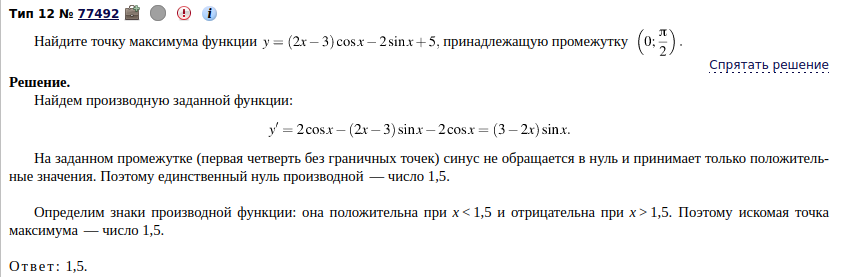
\includegraphics[width=1\linewidth]{VM/ttt.png}
	\end{figure}


\textbf{Код для задачи №77492}


\lstinputlisting{paragrafs/Zadachi/9}

В коде этой задачи не использовалась библиотека \texttt{setMinimaxFunctionTask}, потому что здесь стояла другая цель. Здесь нужно найти точку максимума (минимума) функции, а не её максимальное (минимальное) значение. 

Также здесь присутсвуют подробное поясненяющее решение, которое нельзя было бы получить при использовании библиотеки из прошлой задачи.

\newpage

\textbf{Решения тригонометрической задачи, сгенерированные шаблоном}

	\begin{figure}[h]
		\centering
		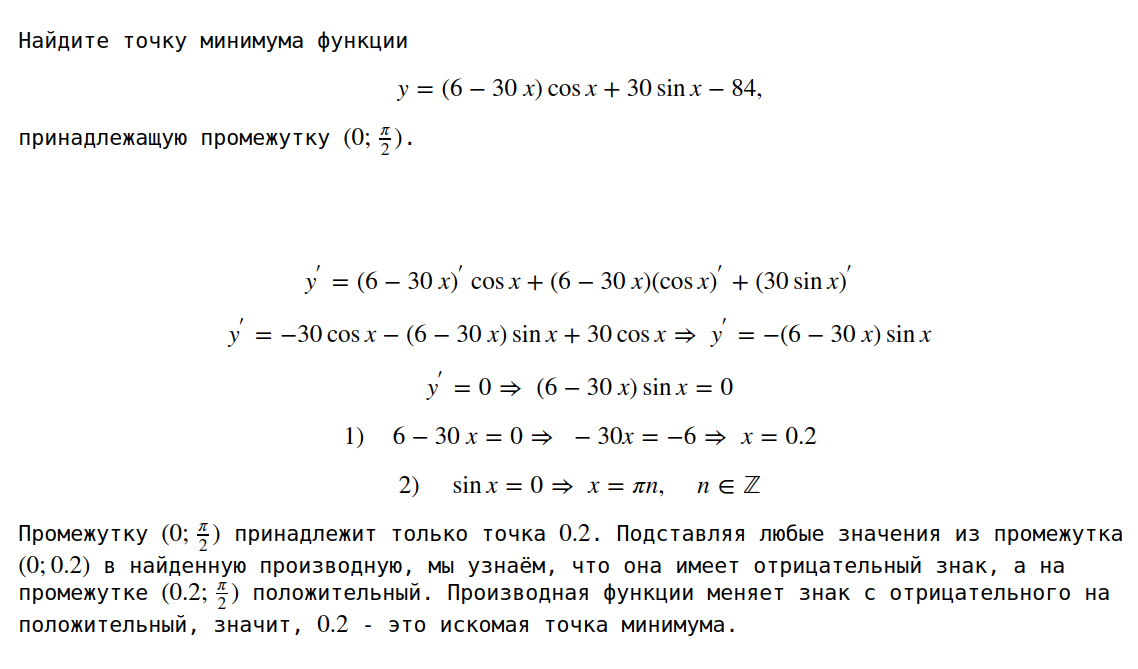
\includegraphics[width=0.8\linewidth]{VM/71.png}
		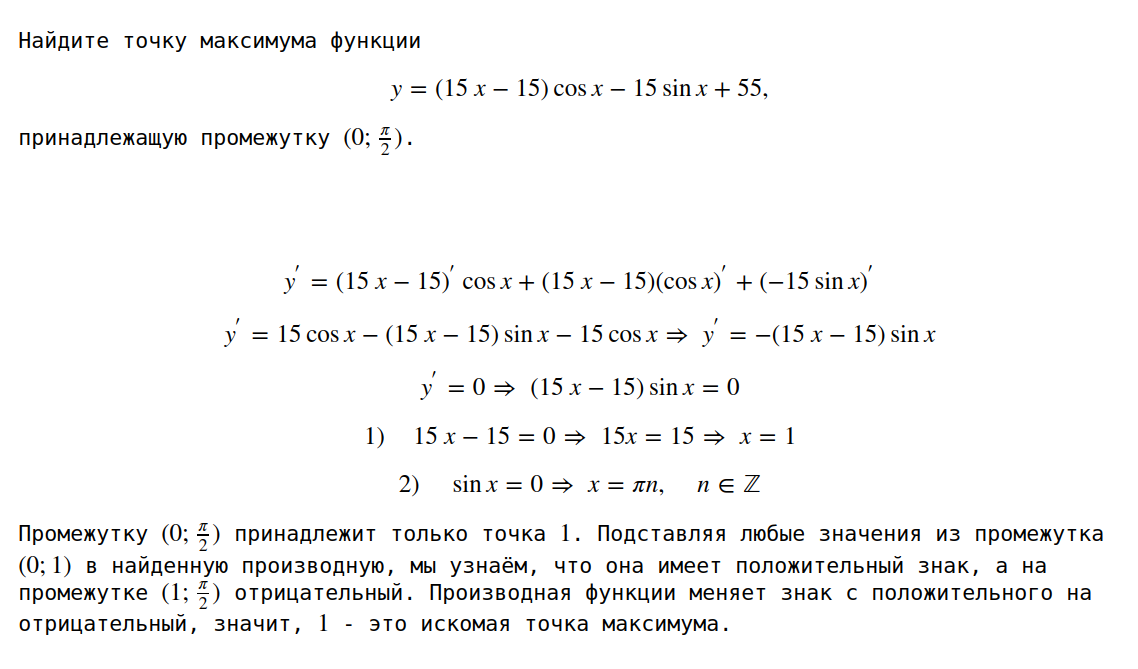
\includegraphics[width=0.8\linewidth]{VM/72.png}
	\end{figure}
	
